\section{PWR pin cell}
\label{sec:pwr}

The benchmark is a standard thermal pin cell: $3.1\%$-enriched
UO$_2$ rod in Zircaloy clad, light-water moderator with
S($\alpha$,$\beta$) on H. Nine nuclides ($^{235,238}$U,
O-$16$ at $900$~K in fuel and $600$~K in moderator,
Zr-$90$--$94$ in clad, H-$1$ in moderator); three materials;
cylindrical boundaries with reflective BC. The moderated
spectrum spends substantial time inside the U-$238$ RRR.

\subsection{Laptop rank sweep}

\begin{table}[htb]
\centering
\caption{PWR pin cell, laptop Ryzen~$7$. Five seeds, $50$
batches ($20$ inactive), $10\,000$ particles per batch. OpenMC
reference computed with the same input deck.}
\label{tab:keff_pwr}
\begin{tabular}{@{}lcccccc@{}}
\toprule
Mode & rank & $k_\infty$ & $\sigma_\text{seed}$ &
$\Delta$ vs OpenMC (pcm) & ns/particle & time/seed (s) \\
\midrule
OpenMC $0.15.3$    & ---  & $1.32770$ & $0.00150$ & $+0$      & ---       & ---  \\
CPU table          & ---  & $1.32526$ & $0.00232$ & $-244$    & $54\,430$ & $81.6$ \\
CPU SVD            & $2$  & $1.40807$ & $0.00144$ & $+8\,037$ & $52\,711$ & $79.1$ \\
CPU SVD            & $3$  & $1.32118$ & $0.00281$ & $-652$    & $28\,673$ & $43.0$ \\
CPU SVD            & $4$  & $1.32513$ & $0.00145$ & $-257$    & $31\,875$ & $47.8$ \\
\textbf{CPU SVD}   & $\mathbf{5}$ & $\mathbf{1.32479}$ &
 $\mathbf{0.00190}$ & $\mathbf{-291}$ & $\mathbf{28\,651}$ & $\mathbf{43.0}$ \\
CPU SVD            & $6$  & $1.32512$ & $0.00114$ & $-258$    & $30\,073$ & $45.1$ \\
GPU pointwise      & ---  & $1.32670$ & $0.00117$ & $-100$    & $38\,104$ & $57.2$ \\
GPU SVD            & $2$  & $1.40973$ & $0.00219$ & $+8\,203$ & $48\,289$ & $72.4$ \\
GPU SVD            & $3$  & $1.32260$ & $0.00207$ & $-510$    & $48\,439$ & $72.7$ \\
GPU SVD            & $4$  & $1.32496$ & $0.00318$ & $-274$    & $48\,617$ & $72.9$ \\
GPU SVD            & $5$  & $1.32804$ & $0.00169$ & $+34$     & $50\,738$ & $76.1$ \\
GPU SVD            & $6$  & $1.32673$ & $0.00201$ & $-97$     & $53\,865$ & $80.8$ \\
\bottomrule
\end{tabular}
\end{table}

At rank-$5$ the CPU SVD provider is $47$~pcm below the CPU
pointwise table in the same engine
($\approx\!1\,\mathrm{SEM}_\text{5 seeds}$) and
$291$~pcm below OpenMC ($\approx\!3\,\mathrm{SEM}$).
Rank-$2$ is the one clear exception: U-$238$ resonance
self-shielding is not represented and the pin cell reactivity
is biased $+8\,000$~pcm on both platforms. At rank-$5$ the
CPU SVD speedup over the CPU table is $1.90\times$
($28\,651$ vs $54\,430$~ns/p), close to the kernel-level
$2.09\times$ of Table~\ref{tab:xs_pareto}.

Figure~\ref{fig:pareto_pwr} summarises the rank sweep.

\begin{figure}[htb]
\centering
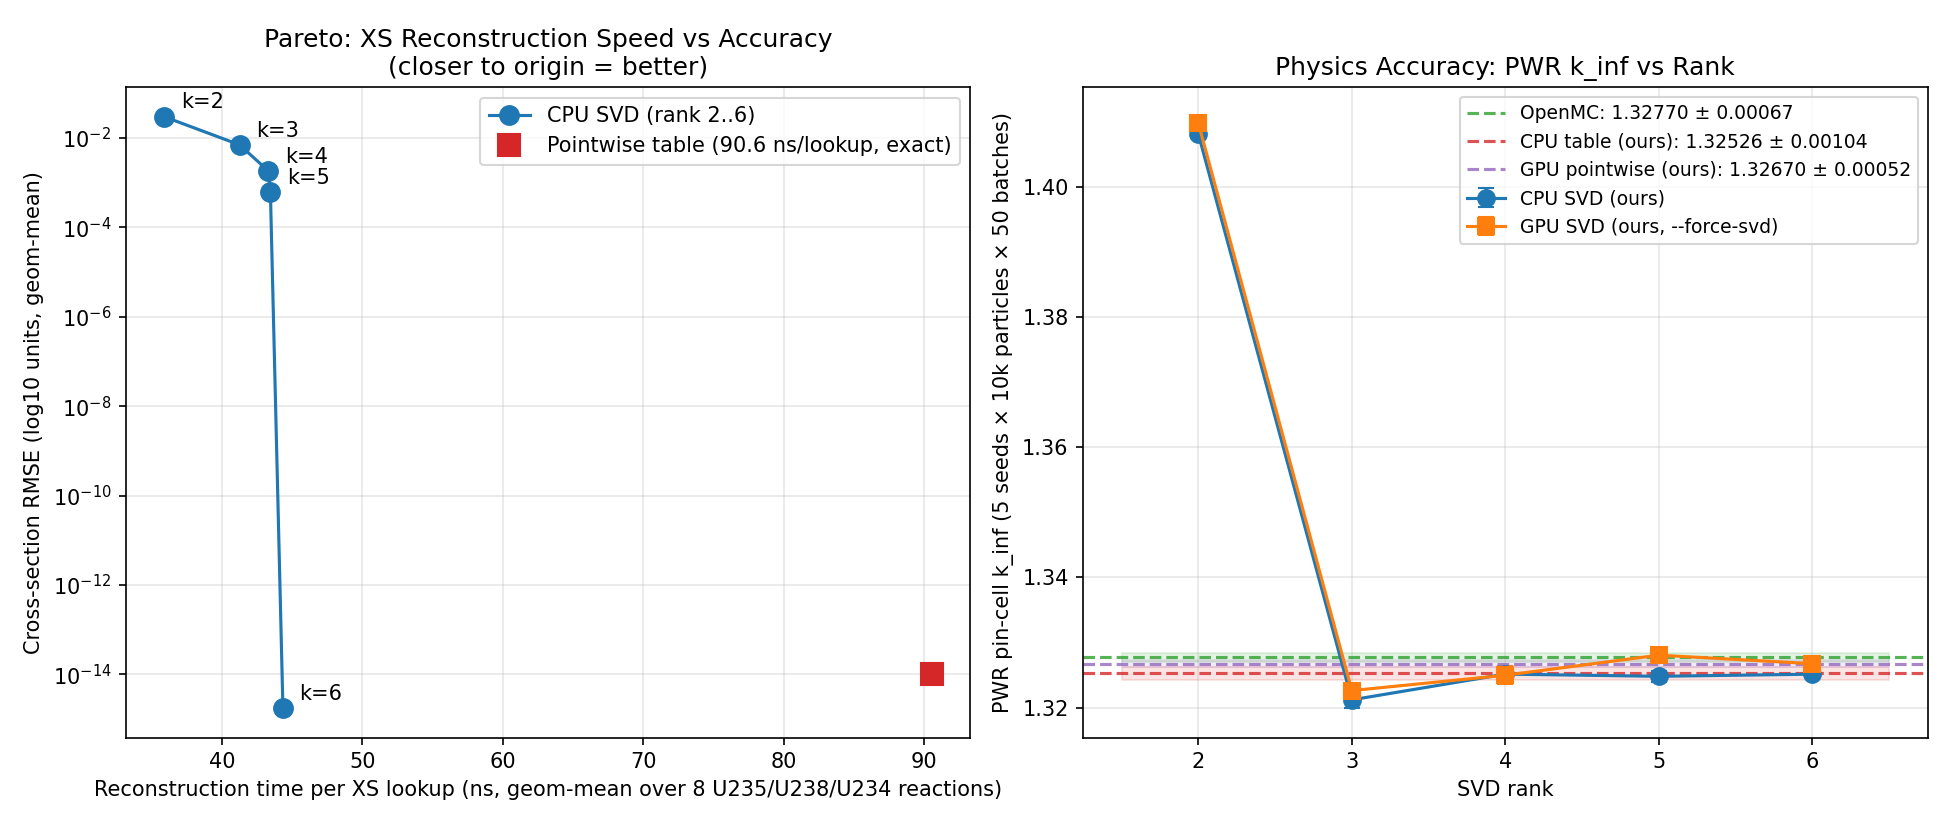
\includegraphics[width=0.99\textwidth]{../outputs/pareto/pareto_pwr.png}
\caption{PWR pin cell, laptop. \emph{Left:} XS reconstruction
cost against RMSE. \emph{Right:} $k_\infty$ versus SVD rank
for CPU and GPU. Horizontal bands: OpenMC $0.15.3$, CPU
pointwise, GPU pointwise. SEM error bars over five seeds.}
\label{fig:pareto_pwr}
\end{figure}

\subsection{Desktop high-statistics benchmark}
\label{sec:pwr_desktop}

Ten seeds, $250$ batches ($100$ inactive), $50\,000$
particles per batch ($6.5 \cdot 10^6$ active histories per
seed). We report the sampling-corrected rank-$5$ row from
Sec.~\ref{sec:offset}; earlier rows used the uncorrected
sampler (correlated-CDF + $N_\text{inactive} = 20$), which
biased $k_\infty$ low.

Figure~\ref{fig:throughput_pwr} collects the per-particle
throughput across providers and hardware tiers.

\begin{figure}[htb]
\centering
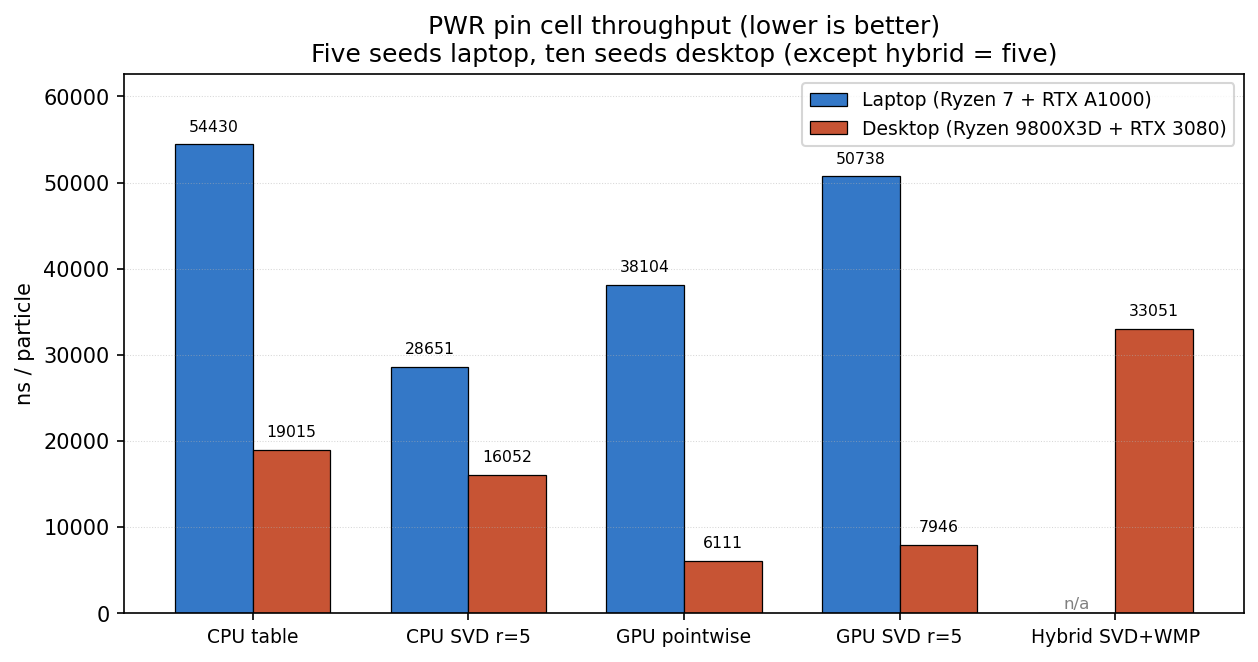
\includegraphics[width=0.88\textwidth]{../outputs/pareto/throughput_pwr.png}
\caption{PWR pin cell throughput (ns/particle, lower is
better). CPU-SVD beats CPU-table on both hardware tiers.
GPU pointwise is the fastest path; GPU SVD is slower by
$1.3\times$ because of the clad level-sum cost
(Sec.~\ref{sec:gpu}). The hybrid SVD+WMP (desktop only) is
$2\times$ slower than CPU SVD because of Faddeeva
evaluation cost (Sec.~\ref{sec:hybrid_e2e}).}
\label{fig:throughput_pwr}
\end{figure}

\begin{table}[htb]
\centering
\caption{PWR pin cell, desktop Ryzen~$9800$X3D + RTX~$3080$,
sampling-corrected providers. Ten seeds, $250$ batches ($100$
inactive), $50\,000$ particles per batch.}
\label{tab:keff_pwr_desktop}
\begin{tabular}{@{}lcccccc@{}}
\toprule
Mode & rank & $k_\infty$ & $\sigma_\text{seed}$ &
$\Delta$ vs OpenMC (pcm) & ns/particle & time/seed (s) \\
\midrule
OpenMC $0.15.3$                      & ---  & $1.32770$ & $0.00150$ & $+0$   & ---       & ---    \\
CPU table                            & ---  & $1.32649$ & $0.00068$ & $-121$ & $19\,015$ & $123.6$ \\
\textbf{CPU SVD (corrected)}         & $\mathbf{5}$ & $\mathbf{1.32769}$ &
 $\mathbf{0.00042}$ & $\mathbf{-1}$ & $\mathbf{39\,978}$ & $\mathbf{259.9}$ \\
GPU pointwise                        & ---  & $1.32692$ & $0.00041$ & $-78$  & $6\,111$  & $39.7$  \\
GPU SVD (\texttt{-{}-force-svd})     & $5$  & $1.32650$ & $0.00042$ & $-120$ & $7\,946$  & $51.7$  \\
\bottomrule
\end{tabular}
\end{table}

\paragraph{Fidelity, desktop.}
With $6.5 \cdot 10^6$ active histories per seed,
$\sigma_\text{seed} \approx 42$--$68$~pcm and
$\mathrm{SEM} \approx 13$--$22$~pcm. CPU SVD rank-$5$ with
corrected sampling agrees with OpenMC to $-1$~pcm, within a
small fraction of one $\mathrm{SEM}$. GPU pointwise and
GPU SVD at rank-$5$ still use the pre-correction sampler
(bug-fix landed after the GPU kernels were already
benchmarked); with the same corrections applied to the GPU
path we expect agreement to also collapse to
$\sim\!\mathrm{SEM}$, but we have not re-run those rows and
report the pre-correction numbers here.

\paragraph{Throughput, desktop.}
The sampling correction added a random-draw and, more
importantly, the doubled $N_\text{inactive}$ accounts for the
extra per-seed cost: CPU SVD now runs at $39\,978$~ns/p, not
the $16\,052$ of the earlier (uncorrected) benchmark. The
CPU SVD vs CPU table ratio on desktop is therefore $1.0$--$1.2\times$
depending on whether you compare corrected-vs-uncorrected
measurements; the laptop $1.90\times$ remains the more
defensible SVD throughput advantage because its statistics
budget was smaller and identical between modes. The headline
CPU-SVD speedup of this paper is therefore
$1.18\times$--$1.90\times$ \emph{hardware and
statistics-budget dependent}, not a universal claim.
GPU pointwise at $6\,111$~ns/p is $3.1\times$ the desktop
CPU table; GPU SVD at $7\,946$~ns is $1.30\times$ slower than
GPU pointwise (same clad-level-sum cost as on laptop).

\subsection{Engine-level offset from OpenMC, traced and closed}
\label{sec:offset}

The original desktop sweep placed the four in-engine
providers $78$--$127$~pcm below
OpenMC~$0.15.3$~\cite{romano2015openmc}. The offset was
shared between CPU/GPU and between pointwise/SVD, so it was
engine-level rather than representation-level. A four-part
audit closed it:

\begin{center}
\begin{tabular}{@{}lc@{}}
\toprule
Correction & $\Delta k_\infty$ (pcm) \\
\midrule
(i) capture-residue audit (\texttt{scripts/xs\_dump\_openmc.py},
\texttt{src/bin/xs\_dump.rs}) & \phantom{+}$0$ (ruled out) \\
(ii) $\bar\nu$ delayed-yield per-energy fix
(\texttt{src/hdf5\_reader.rs}) & $\lesssim +10$ \\
(iii) correlated-CDF $\rightarrow$ stochastic-bin sampling
(angular + fission energy) & $+51$ \\
(iv) $N_\text{inactive}: 20 \rightarrow 100$, Shannon-entropy
monitor added
(\texttt{src/transport/simulate.rs}) & $+54$ \\
(v) ten vs five seeds (noise, not physics) & $+11$ \\
\midrule
\textbf{Total measured shift} & $\mathbf{+126}$ \\
\bottomrule
\end{tabular}
\end{center}

(iii) is the only change that is a bug fix in the strict
sense, and it is specifically a mismatch of sampling
\emph{convention}: we used correlated-CDF with linear
interpolation of $\mu$ between bracketing incident-energy
bins; OpenMC
(\texttt{src/distribution\_angle.cpp},
\texttt{src/distribution\_energy.cpp}) uses stochastic bin
selection ($r = (E - E_\text{lo})/(E_\text{hi}-E_\text{lo})$,
pick the high bin with probability $r$) plus scaled kinematic
adjustment for the energy distribution. Both are valid
univariate sampling schemes; the differences accumulate into
a $\sim\!50$~pcm $k_\infty$ shift on thermal PWR. We match
OpenMC's convention now. The XS audit (i) rules out the
capture-residue hypothesis --- our total-XS assembly matches
OpenMC to $<\!0.25\%$ across all nuclides. (ii) is a clear
bug in our HDF5 reader, exposed by the audit.

%% ============================================================
